\begin{figure}[!t]
    \centering
    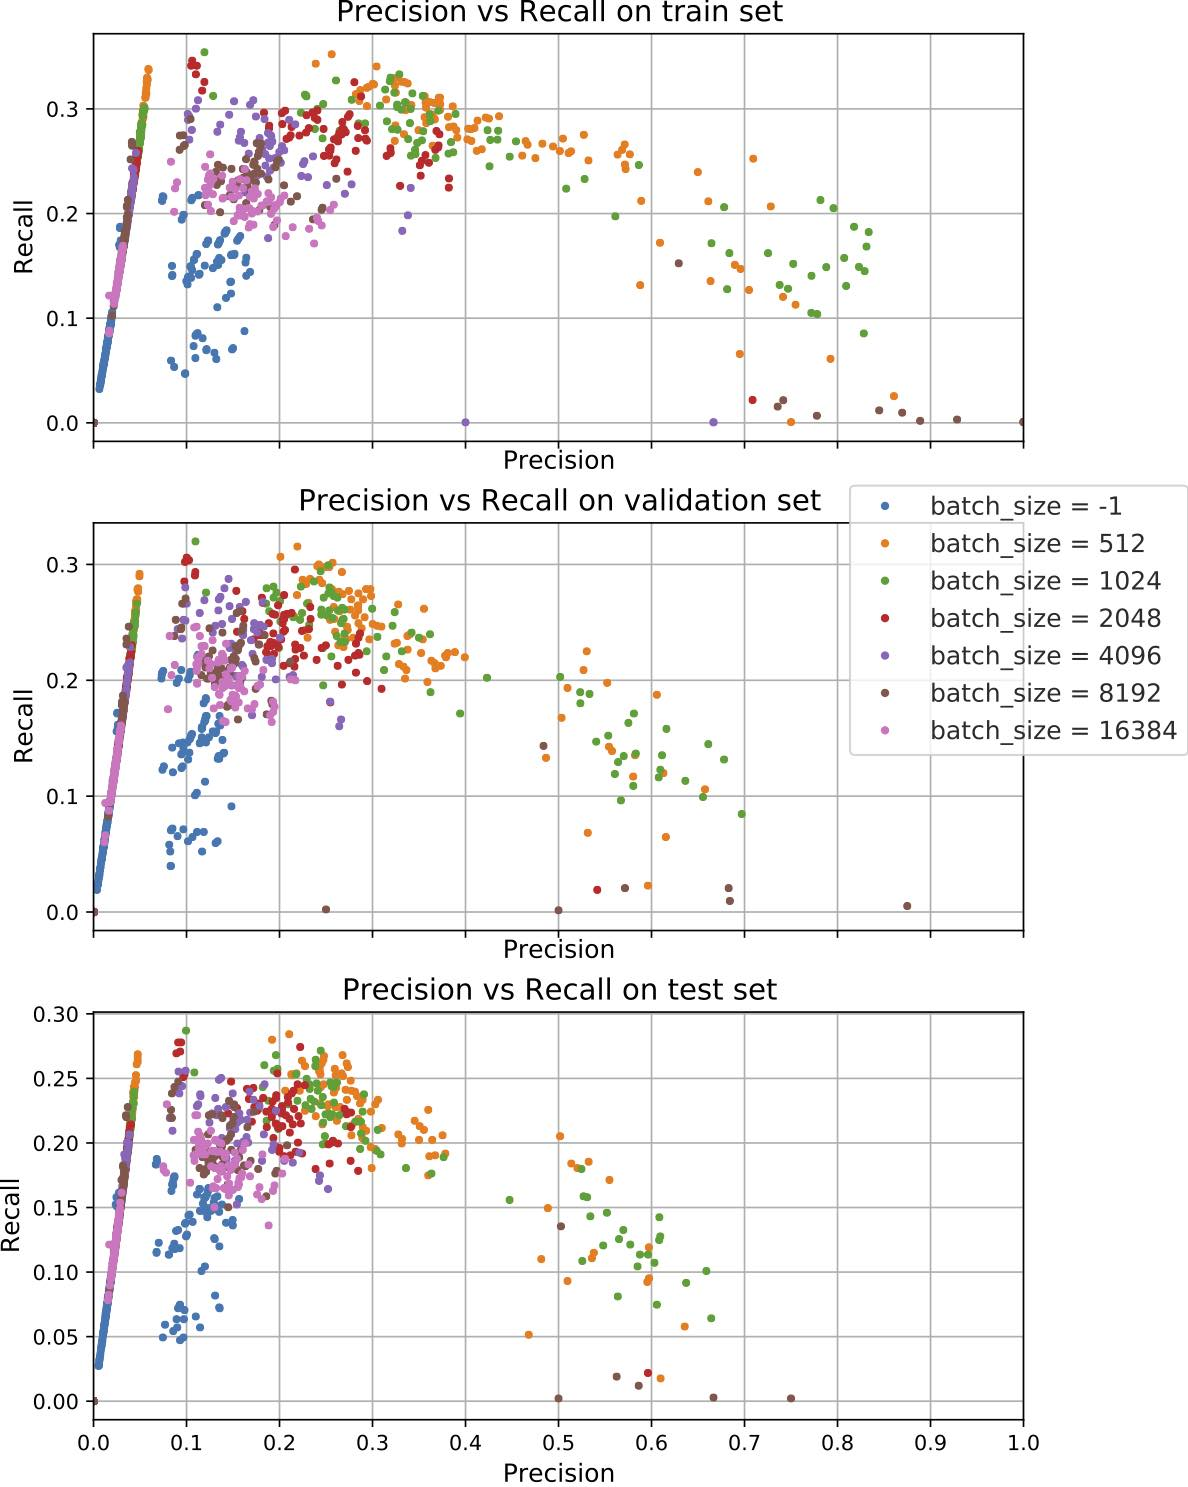
\includegraphics[height=0.9\textwidth]{content/chapters/false_alarm_control/figures/precision_recalls_batch_sizes.jpg}
    \caption[Sigmoid bound objective's sensitivity to batch size]{Sensitivity of precision and recall as we vary the batch size from 512 up to the size of the entire training set. Rows show the training, validation, and test set performance on the MIMIC-III dataset mortality risk prediction task.
    Each dot represents the performance of one run of our sigmoid bound method optimized to convergence from one random initialization; we plot many runs for each batch-size setting to show the range of possible local optima. The best runs with batch sizes of 512 and 1024 surpass the best runs at any other tested batch size, as shown by the cluster of orange and green points that reach 0.45-0.75 precision and 0.18-0.26 recall on the test set, when training with the precision constraint, $\alpha=0.7$. Batch size = -1 indicates the full training set.
    }%endcaption
    \label{fig:batch_size_sensitivity}
\end{figure}